\section{Examples of derivable functions}\label{sec:AppendixExamples}
To illustrate derivable functions, we present a series of examples, some of them will be useful later.

\noindent \begin{example}[Identity] For every type $\rSigma$, the identity function $x\in\rSigma\mapsto x\in\rSigma$ is derivable. This is achieved by induction on the types: the identity function over a finite set of elements is derivable since its domain is finite. %, and the identity function over $\llone$ is the first-order function $!$.
For every types $\rSigma$ and $\rGamma$, the identity
function over $\ranked{\rSigma+\rGamma}$ is the disjoint union of the co-projections $\ranked{\rSigma \to \rSigma + \rGamma}$ and $\ranked{\rGamma \to \rSigma + \rGamma}$. The
identity function over $\ranked{\rSigma \times \rGamma}$ is the pairing of the projections $\ranked{\rSigma \times \rGamma \to \rSigma}$ and $\ranked {\rSigma \times \rGamma \to \rGamma}$. The
identity function over $\ranked{\rSigma \otimes \rGamma}$ is the tensor product of the identity over $\rSigma$ and the identity over $\rGamma$. Finally,
the identity function over $\tmonad\rSigma$ and $\reduce k$ are constructed from the identity function over $\rSigma$ using the combinators $\tmonad$ and $\reduce k$ respectively.
\end{example}


\medskip
\noindent\begin{example}[Filter]\label{ex:filter} Consider the types $\rGamma, \rSigma$  where $\rGamma$ is a finite type of unary symbols. Consider the function:
$$ \ranked{f:\tmonad (\rSigma+\rGamma)\to\tmonad \rSigma}$$
which erases the elements of $\rGamma$ from the inupt tree. This function is well defined since erasing unary symbols does not break the tree structure of the input. 
Let us explain why this is a derivable function. 
Consider the basic functions $\ranked{\unit_\rSigma:\rSigma\to\tmonad\rSigma}$ and the constant function $\ranked{\mathsf{empty}:\rGamma\to\tmonad\rSigma}$ which associates to every element of $\rGamma$ the tree reduced to the variable $x_1$. Using the cases combinator, we get a tree in $\tmonad\tmonad\rSigma$, which we transform into a tree in $\tmonad \rSigma$ using the flattening function $\flatt_\rSigma$.
\end{example}
\medskip

\noindent \begin{example}[Pattern matching]\label{ex:patternMatching} 
\end{example}
\medskip

\noindent \begin{example}[Tree homomorphisms]\label{ex:morphism} 
Given two types $\rSigma, \rGamma$ and an arity preserving  function $\ranked{f:\Sigma\to\tmonad\Gamma}$, we can lift $\ranked{f}$ to the tree homomophism  $\ranked{\mathsf{Hom}_f:\tmonad\Sigma\to \tmonad\Gamma}$ which replaces every node by the term corresponding to its label. If $\ranked{f}$ is derivable, then so is  $\mathsf{Hom}_f$. To see this, we use the composition of the two basic functions
\begin{align*}
\ranked{\tmonad\Sigma\xrightarrow{\tmonad f}\tmonad\tmonad\Gamma \xrightarrow{\flatt_\Gamma} \tmonad \Gamma}
\end{align*} 
\end{example}
\medskip

\noindent \begin{example}[Parent and sibling informations]\label{ex:sibling}  Let $\rGamma$ be a finite type. We define $\ranked{\rGamma_0}$  to be the ranked set obtained from $\rGamma$ by setting the arity of every element to $0$.  
\medskip
Consider the function:
$$\ranked{ \mathsf{Parent}: \tmonad \rGamma \to \tmonad (\rGamma\otimes (\rGamma+\bot)_0)}$$
which adds to every node of a term in $\tmonad \rSigma$ the label  of its parent if it has one and $\bot$ if it is the root.

% from  $(\rGamma\cup\bot)^{\leq n}$, whose lenght is the arity of the node, and such that the $i^{th}$ element of the  list is the symbol of its $i^{th}$ sibling if it has one, otherwise it is $\bot$.
Let us explain how $\ranked{\mathsf{Parent}}$ can be derived. To illustrate this construction, we use the ranked alphabet and the term below as running examples of the alphabet $\rGamma$ and a term in $\tmonad\rGamma$.
\begin{center}
		Example of the alphabet $\rGamma$
		
		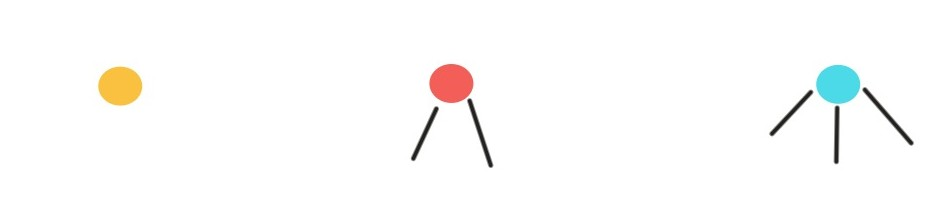
\includegraphics[scale=.15]{MyPic0.jpg}
		
		Example of a term in $\tmonad \rGamma$
		
		 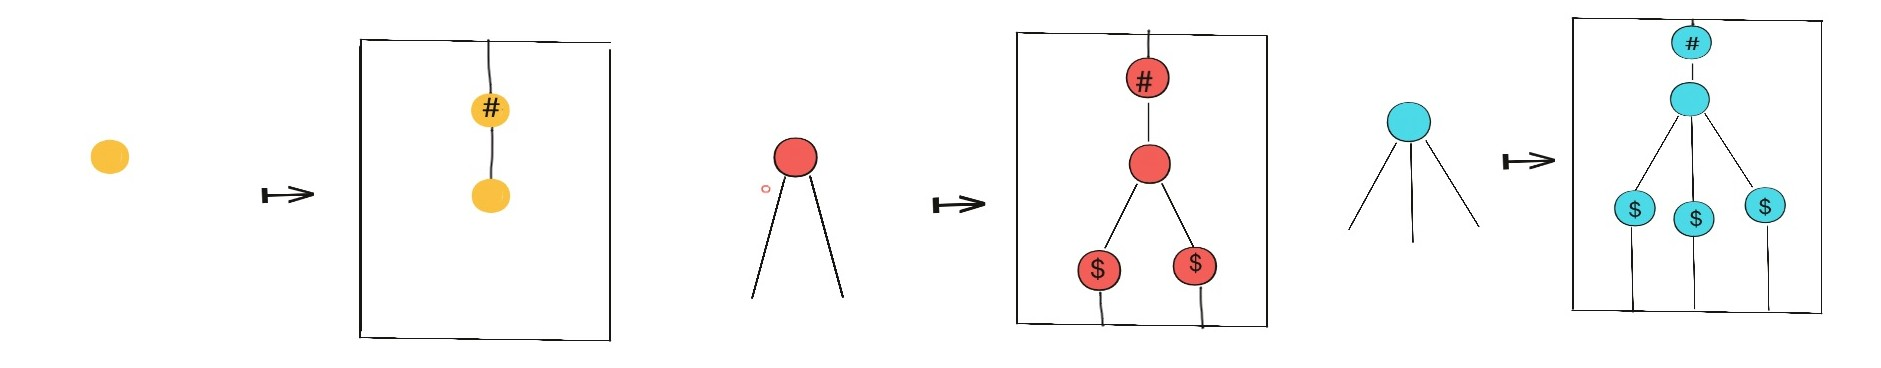
\includegraphics[scale=.15]{MyPic1.jpg}
		\end{center}
We denote by $\ranked{\Gamma_1}$ the ranked set obtained from $\rGamma$ by setting the arity of every element to $1$. If $a$ is a element of $\rGamma$, we denote by $a_1$ the corresponding element of $\ranked{\Gamma_1}$. In our example, the alphabet $\ranked{\Gamma_1}$ is
\begin{center}
		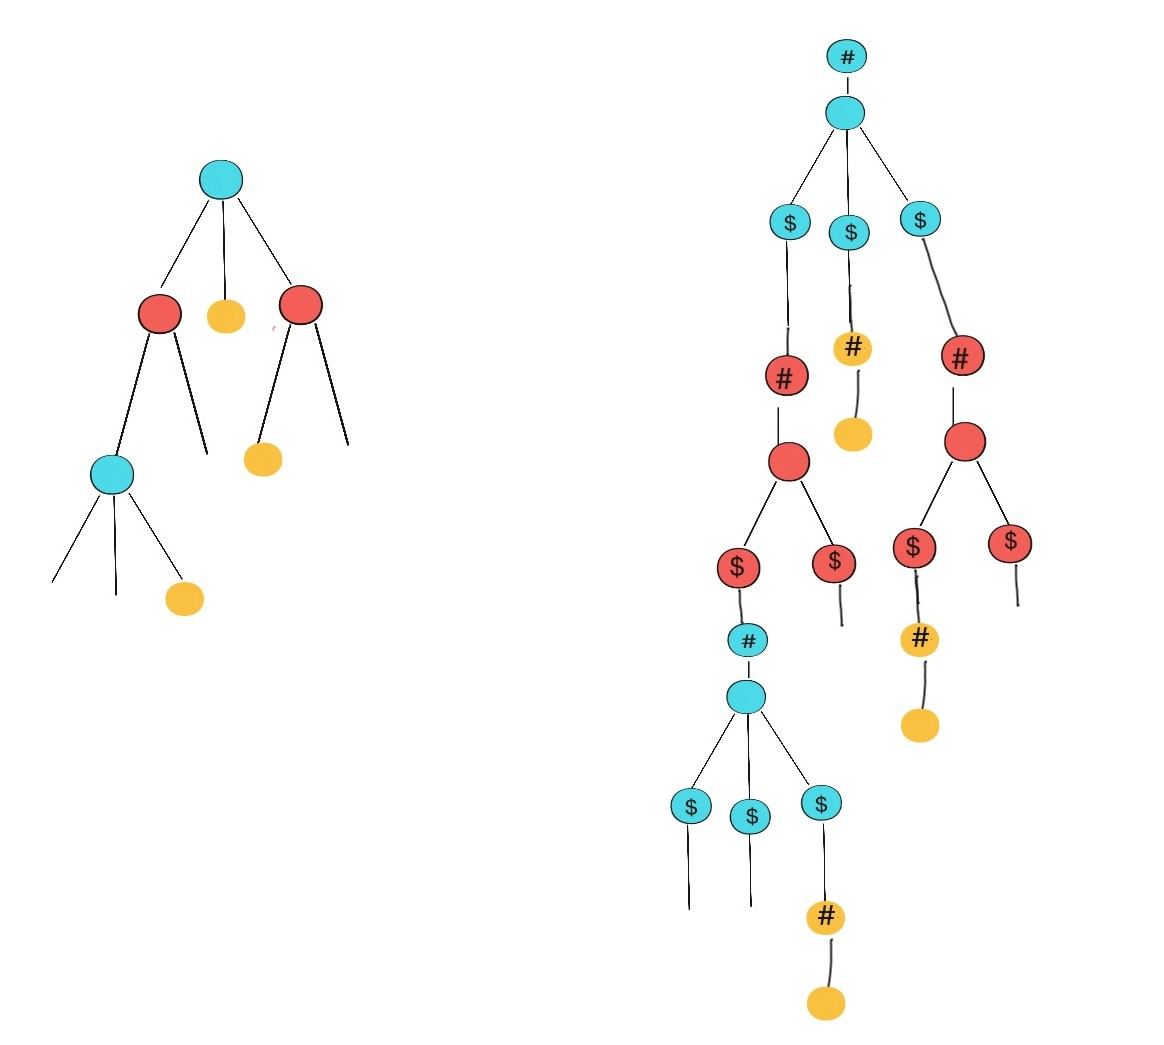
\includegraphics[scale=.15]{MyPic2.jpg}
		\end{center}
\begin{enumerate}
\item  First, we apply the homomorphism 
\begin{align*}
\ranked{\mathsf{Hom}_g:\tmonad\Gamma\to \tmonad(\Gamma+\Gamma_1+\set{\#})}
\end{align*}
where $\#$ is a unary symbol, and $\ranked{g}$ is defined on the elements of $\Gamma$ as follows
\begin{align*}
\ranked{g: \Gamma} & \ranked{\to  \tmonad(\Gamma+\Gamma_1+\set{\#} )}\\
      a & \mapsto a\tensorpair{\#\tensorpair{a_1\tensorpair{x_1}},\dots, \#\tensorpair{a_1\tensorpair{x_n}}}\qquad n=\arity a
\end{align*}
In our example, the action of $\ranked{g}$ on the elements of $\rGamma$ looks like this
\begin{center}
		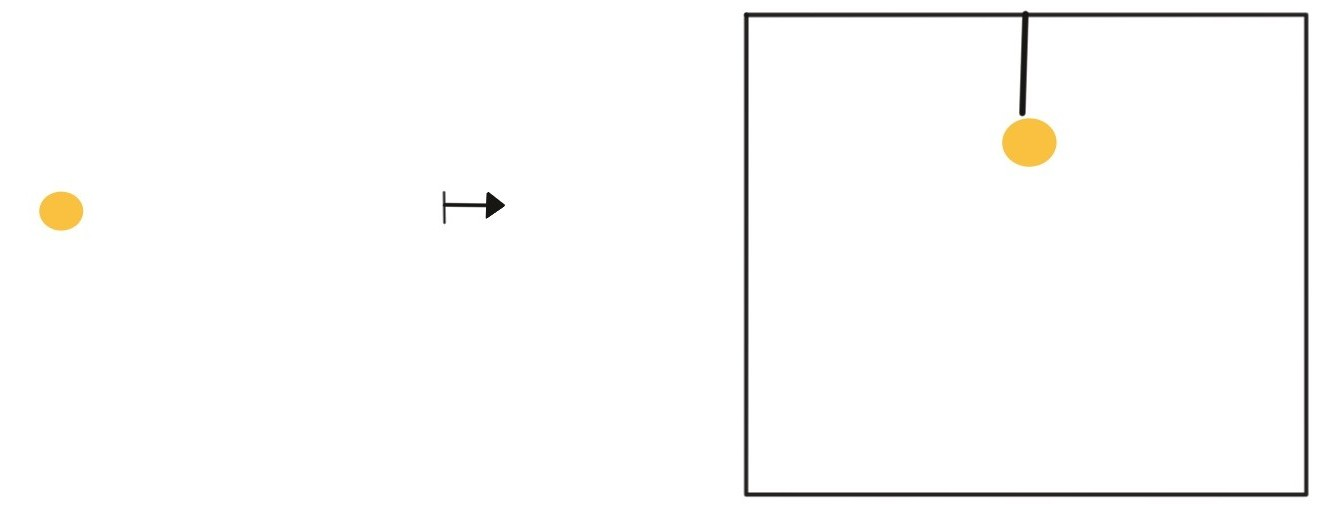
\includegraphics[scale=.1]{MyPic3a.jpg}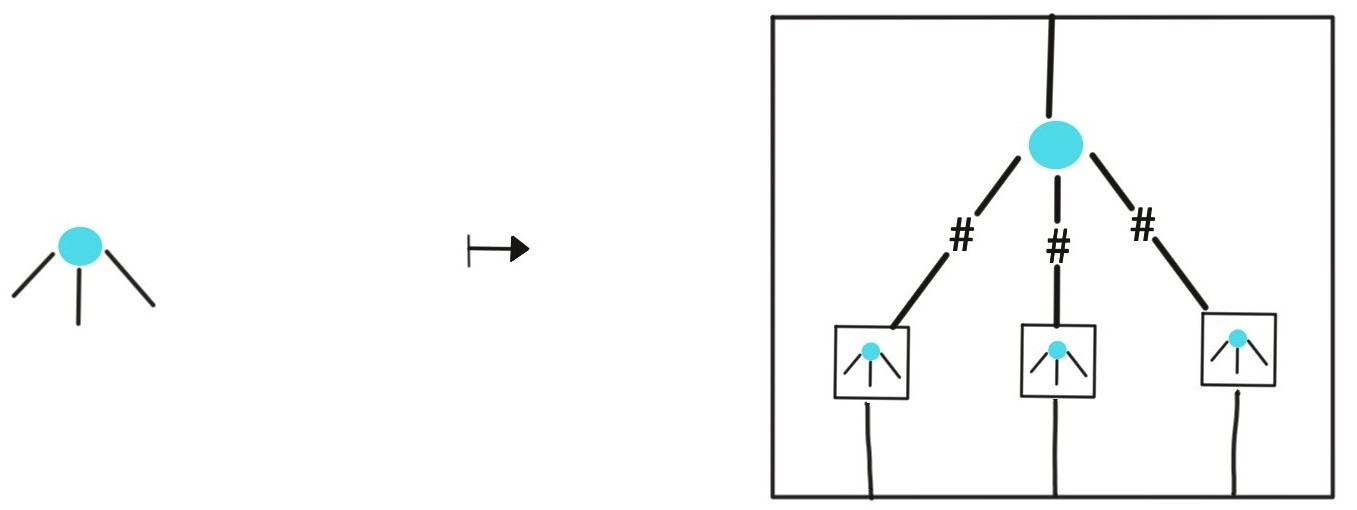
\includegraphics[scale=.1]{MyPic3b.jpg}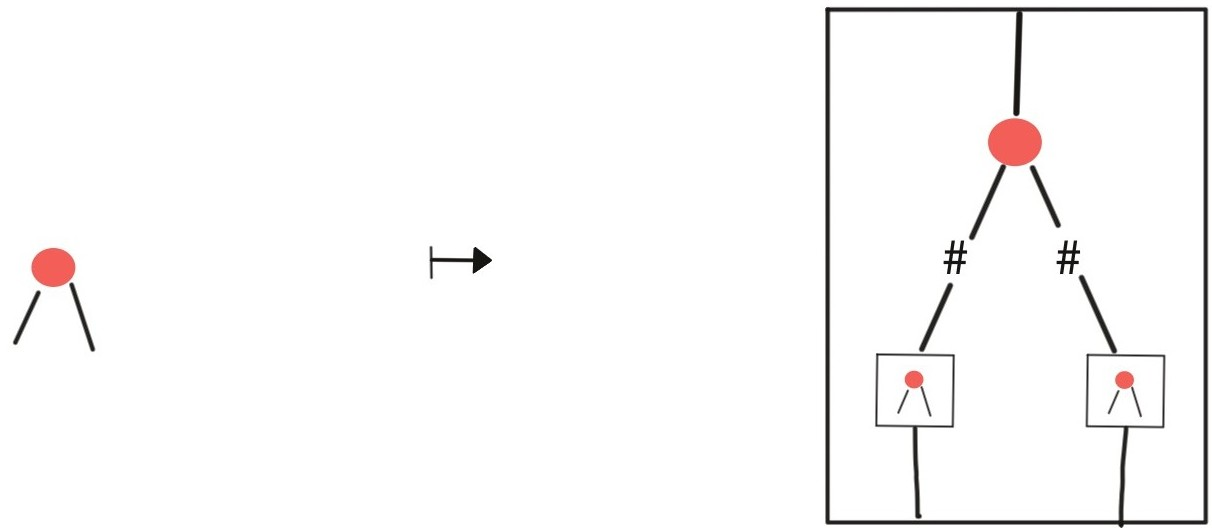
\includegraphics[scale=.1]{MyPic3c.jpg}
		\end{center}
Hence, after the application of the homomorphism $\ranked{\mathsf{Hom}_g}$, our initial term becoms
\begin{center}
		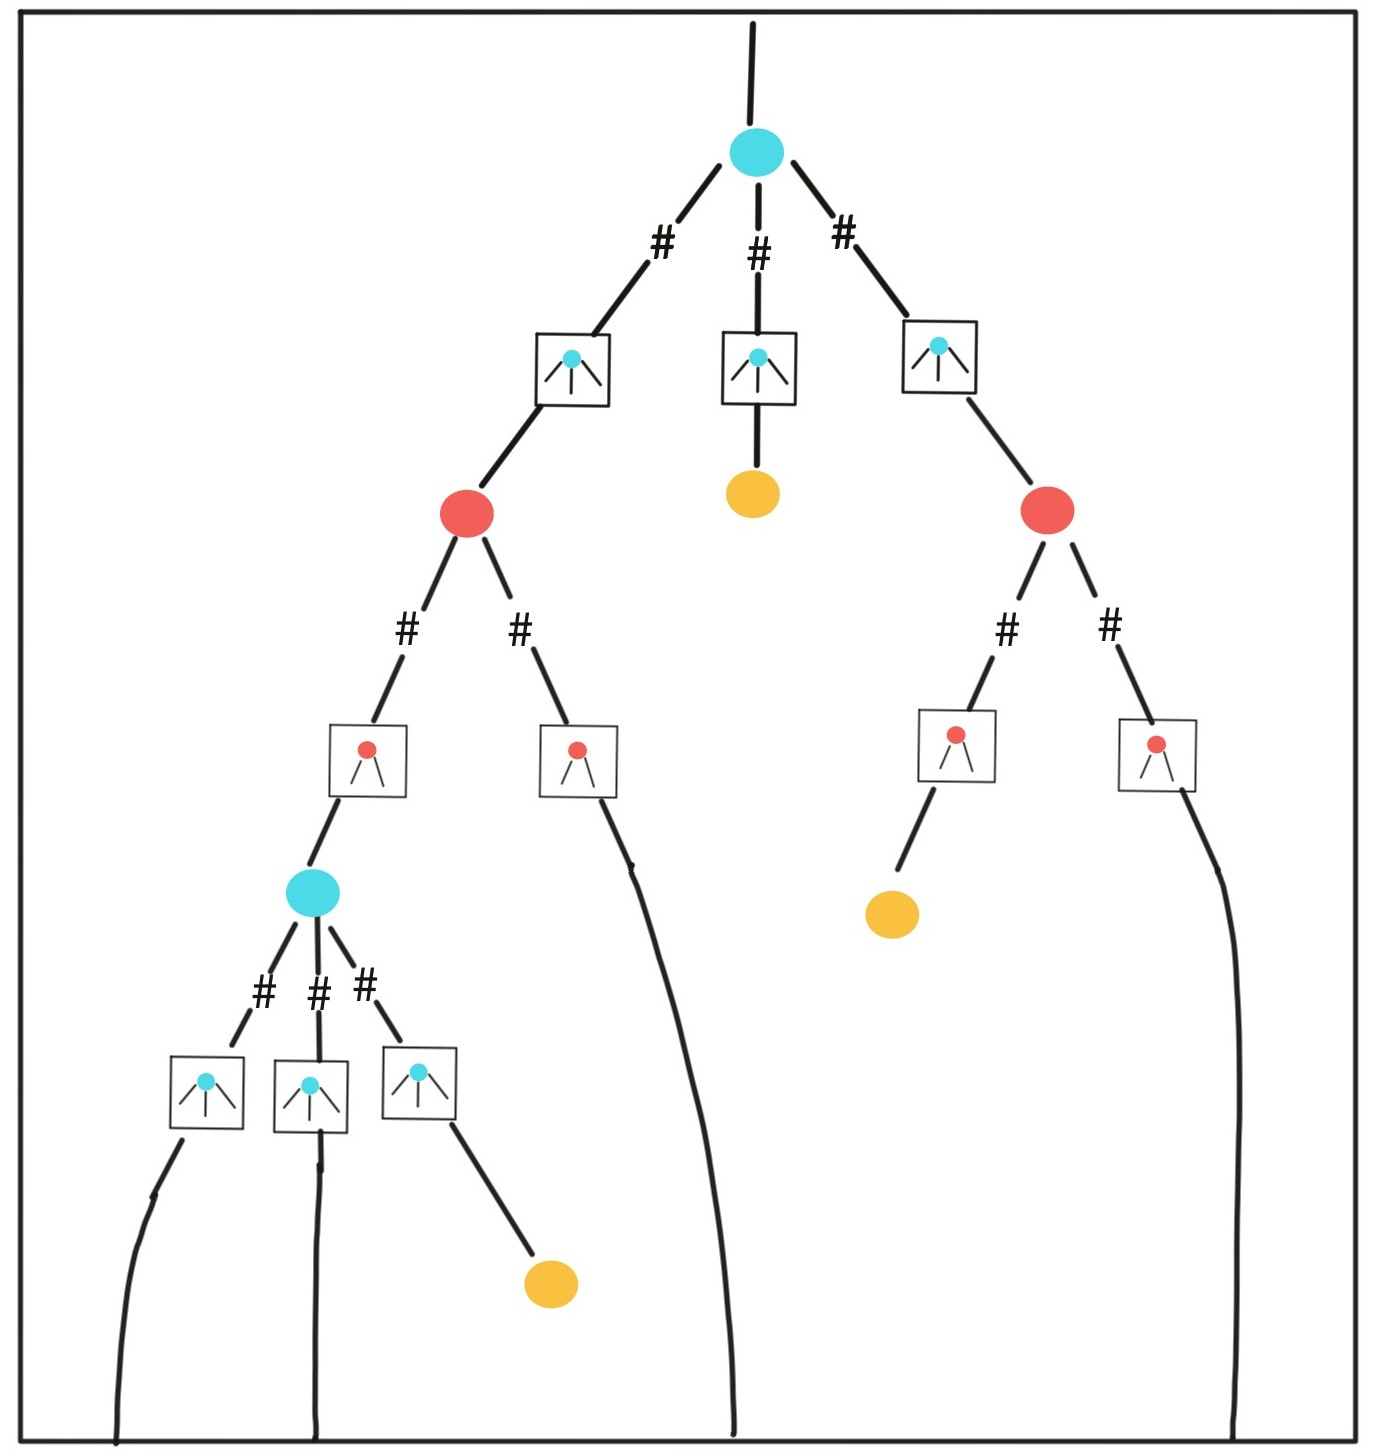
\includegraphics[scale=.15]{MyPic4.jpg}
		\end{center}
\item We apply the factorsation 
\begin{align*}
\ranked{\ancfact: \tmonad(\Gamma+\Gamma_1+\set{\#}) \to \tmonad(\tmonad(\Gamma+\Gamma_1)+\tmonad\set{\#})}
\end{align*}
 to separate the symbol $\#$ form the other symbols. After this operation, each node lies in the same factor as (the element of $\ranked{\Gamma_1}$ representing) its parent. In our example, the obtained term is the following
\begin{center}
		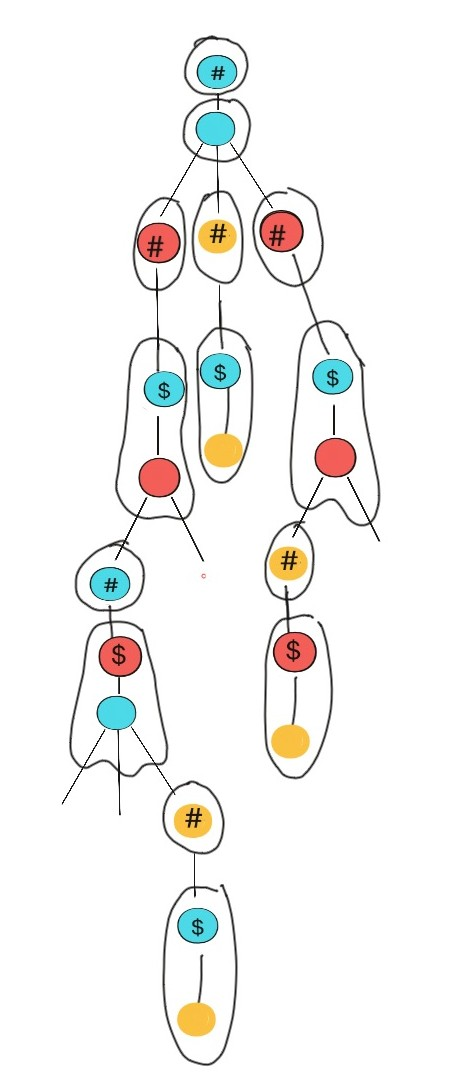
\includegraphics[scale=.15]{MyPic5.jpg}
		\end{center}
\item Consider the function 
\begin{align*}
\ranked{h: \tmonad\set{\#} \to \tmonad(\Gamma+\Gamma_1+(\Gamma+\bot)_0)}
\end{align*}
which is the constant function equal to the empty term (that is the term $x_1$).
And let $k$ be the function
\begin{align*}
\ranked{k: \tmonad(\Gamma+\Gamma_1) \to \tmonad(\Gamma+\Gamma_1+(\Gamma+\bot)_0)}
\end{align*}
which is the identity function, execpt for the follonwing terms in which it is defined as follows
$$\begin{array}{rll}
a\tensorpair{x_1,\dots, x_n}& \mapsto & \tensorpair{a,\bot}\tensorpair{x_1,\dots,x_n}\qquad n=\arity(a)\\
b_1\tensorpair{a\tensorpair{x_1,\dots,x_n}}&\mapsto& \tensorpair{a,b}\tensorpair{x_1,\dots,x_n}\\
b_1\tensorpair{x_1} &\mapsto& x_1
\end{array}$$
\end{enumerate}
	

\medskip
If $\rGamma$ is a finite ranked set, we define $\ranked{\Gamma^*}$ as
$$\ranked{\coprod_{i \leq \text{ maximal arity in } \rGamma} \underbrace{\rGamma\otimes \cdots \otimes \rGamma}_{i\text{ times}}}$$
Now consider the function $$\ranked{\mathsf{Sibling}:\tmonad\rGamma\to \tmonad (\rGamma\otimes (\rGamma+\bot)^*_0)}$$ which taggs every node of a term in $\tmonad \rSigma$ by the list  of its children symbols. When a child is a port, it is marked by $\bot$ in the list.
The fuction $\ranked{\mathsf{Sibling}}$ is derivable. To see this, the same steps above can be followed, exept for steps 6 and 7 which should be adapted to this case. 
\end{example}



\medskip
\noindent  \begin{example}[Root and leaves] Let $\rSigma$ be a finite type and $f:\rSigma \to \rGamma$, $g: \rSigma \to \rGamma$ be derivable functions. The function $$\ranked{\mathsf{Root}_{f,g} : \tmonad\rSigma \to \tmonad\rGamma}$$
which applies $f$ to the root and $g$ to the rest of the tree is a derivable function.
 
To show this, we first start by applying the function $\ranked{\mathsf{Parent}:\tmonad\rSigma\to\tmonad(\rSigma\otimes(\rSigma+\bot)_0)}$. Doing so, the root can be distinghished from the other nodes since it will be tagged by $\bot$.  

The function $\ranked{h}$ defined by 
\begin{align*}
\ranked{h:\rSigma\otimes(\rSigma+\bot)_0}&\ranked{\to \rGamma}\\
  \tensorpair{a,\bot} &\mapsto f(a) \\
  \tensorpair{a,b} &\mapsto g(a) \text{ if } b\neq \bot.
\end{align*}
is derivable since its domain is finite. 
We lift $h$ to terms of $\tmonad\rGamma$ to conclude.


%We lift the function $ditribute_\otimes: \rSigma\otimes\rSigma^{\leq 1}\to  \rSigma\otimes\rSigma^{=0}+ \rSigma\otimes\rSigma^{= 1}$ to the trees of $\tmonad \rSigma\otimes\rSigma^{\leq 1}$ to get trees in $\tmonad (\)$.

\medskip
The function $$\ranked{\mathsf{Leaves}_{f,g} : \tmonad\rSigma \to \tmonad\rGamma}$$
 which applies $f$ to the leaves and $g$ to the rest of the tree is derivable. This is done using the same ideas as before, but invoquing the function $\ranked{\mathsf{Sibling}}$ instead of the function $\ranked{\mathsf{Parent}}$: leaves can be distingushed from the other nodes since they are tagged either by a list of $\bot$ or the empty list.
\end{example}

\medskip
\noindent\begin{example}[Descendent and ancestors]\label{ex:descendant} If $\rSigma$ is a finite type and $\rGamma\subseteq \rSigma$, then the functions 
\begin{itemize}
\item $\ranked{\mathsf{Descendant}_\rGamma: \tmonad \rSigma \to \tmonad (\rSigma+\rSigma)}$ which replaces the label of each node by its first or second copy, depending on whether it has a descendent in $\rGamma$,
\item $\ranked{\mathsf{Ancestor}_\rGamma: \tmonad \rSigma \to \tmonad (\rSigma+\rSigma)}$ which replaces the label of each node by its first or second copy, depending on whether it has a descendent in $\rGamma$,
\end{itemize}
are derivable.

To derive $\ranked{\mathsf{Descendant}_\rGamma}$, we start by applying the factorisation $$\ranked{\decfact: \tmonad\rSigma\to \tmonad(\tmonad\rGamma+\tmonad(\rSigma\setminus\rGamma))}$$ which regroups the elements of $\rSigma$ and the elements of $\ranked{\rSigma\setminus\rGamma}$ into factors, as in the following figure, where $\rGamma$ is represented by the blue nodes and $\ranked{\rSigma\setminus \rGamma}$ by the red ones:
\begin{center}
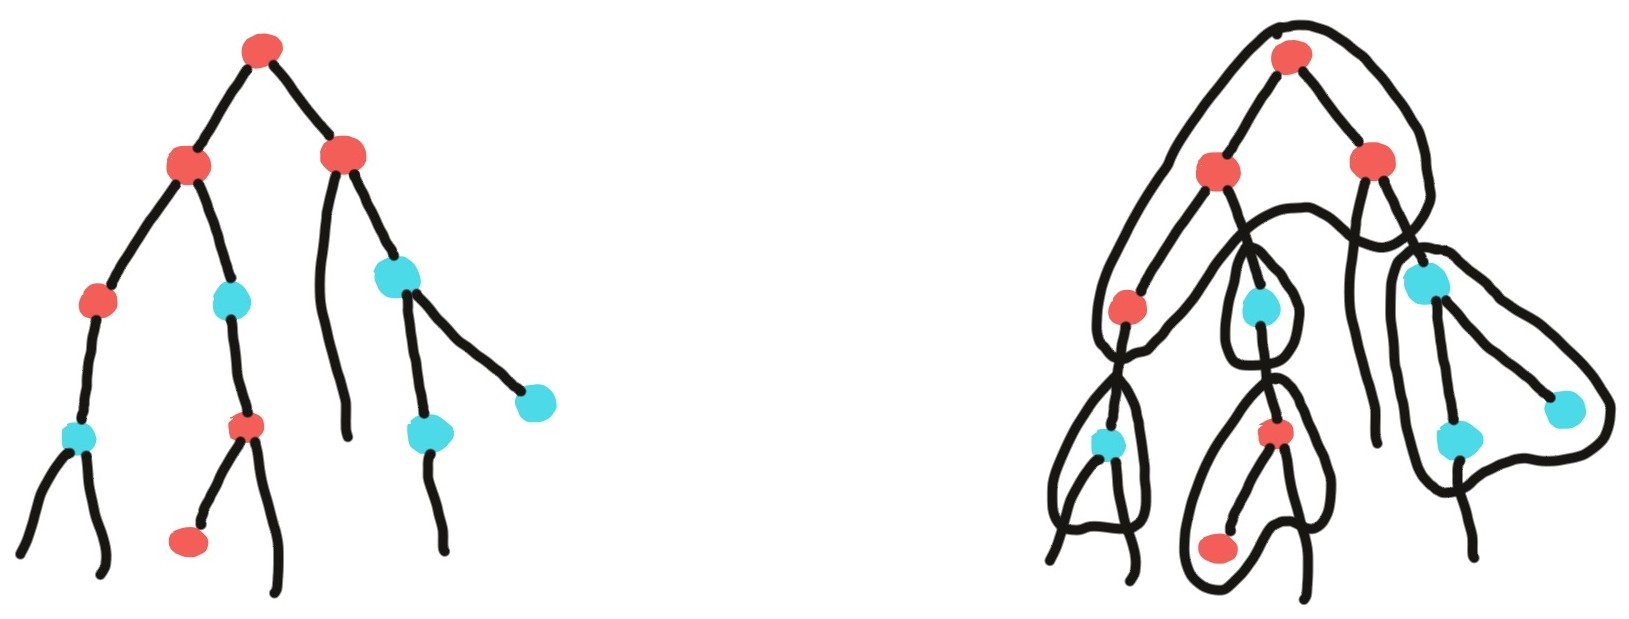
\includegraphics[scale=.15]{MyPic6.jpg}
\end{center}
Obviously, all the nodes of the $\Gamma$ factors have a descendant in $\rGamma$. 
In the $\ranked{\rSigma\setminus\rGamma}$ factors which are not leaves in the factorized term, all the nodes have a $\rGamma$ descendant in the original term. To show this, take $f$ to be one of these factors, and suppose by contradiction that one of its nodes does not have a descendant in $\rGamma$. By definition of $\ancfact$, all the elements of $f$ do not have a descendant in $\rGamma$ as well. Since $f$ is not a leaf, it has a child $g$. The factor $g$ cannot be a $\rGamma$
factor as the nodes of $f$ would have a descendant in $\rGamma$. The factor $g$ is then necessarily  a $\ranked{\rSigma\setminus \rGamma}$ factor. If a node of $g$ has a descendant in $\rGamma$, this would give a $\rGamma$ descendant to one of the node of $f$. Thus all the nodes of $g$ are in $\ranked{\rSigma\setminus \rGamma}$ and do not have a descendant in $\rGamma$, meaning that $f$ and $g$ are actually the same factor, which gives a contradiction. Finally, the $\ranked{\rSigma\setminus\rGamma}$ factors which are leaves do not have a descendant in $\rGamma$. With these observations, we can now implement $\mathsf{Descendant}_\rGamma$. 

Let us consider the functions 
$$\begin{array}{llll}
\ranked{\mathsf{Yes}_\rGamma :} & \rGamma &\ranked{\to} &\ranked{ \rSigma+\rSigma}\\
 \ranked{\mathsf{Yes}_{\ranked{\rSigma\setminus\rGamma}:}}& \ranked{\rSigma\setminus\rGamma}&\ranked{\to} &\ranked{ \rSigma+\rSigma}\\
\ranked{\mathsf{No}_{\ranked{\rSigma\setminus\rGamma}: }}&\ranked{\rSigma\setminus\rGamma} &\ranked{\to}& \ranked{ \rSigma+\rSigma}
\end{array}$$
which replaces the label of each node by its first copy for $\ranked{\mathsf{Yes}_\Gamma}$ and $\ranked{\mathsf{Yes}_{\rSigma\setminus\rGamma}}$, and by its second copy for $\ranked{\mathsf{No}_{\rSigma\setminus\rGamma}}$. The three functions are derivable as their domains are finite. 
Consider the functions 
\begin{align*}
\ranked{f} &\ranked{: \tmonad\rGamma+\tmonad(\rSigma\setminus\rGamma) \to \tmonad (\rSigma+\rSigma)}\\
&=\ranked{ \tmonad\mathsf{Yes}_\rGamma \text{ or } \tmonad\mathsf{No}_{\rSigma\setminus \rGamma}}\\
\ranked{g} &\ranked{: \tmonad\rGamma+\tmonad(\rSigma\setminus\rGamma) \to \tmonad (\rSigma+\rSigma)}\\
&=\ranked{ \tmonad\mathsf{Yes}_\rGamma \text{ or } \tmonad\mathsf{Yes}_{\rSigma\setminus \rGamma}} 
\end{align*}
The descendant function is obtained by applying $\ranked{\mathsf{leaves}_{f,g}}$ followed by a flattening.

To derive the function $\ranked{\mathsf{Ancestor}_\Gamma}$, we apply first a the factorisation
$$\ranked{\ancfact: \tmonad\rSigma\to \tmonad(\tmonad\rGamma+\tmonad(\rSigma\setminus\rGamma))}$$ which regroups the elements of $\rSigma$ and the elements of $\ranked{\rSigma\setminus\rGamma}$ into factors depending on whether they have the same descendant of the same type. Here is an example,  where $\rGamma$ is represented by the blue nodes and $\ranked{\rSigma\setminus \rGamma}$ by the red ones:
\begin{center}
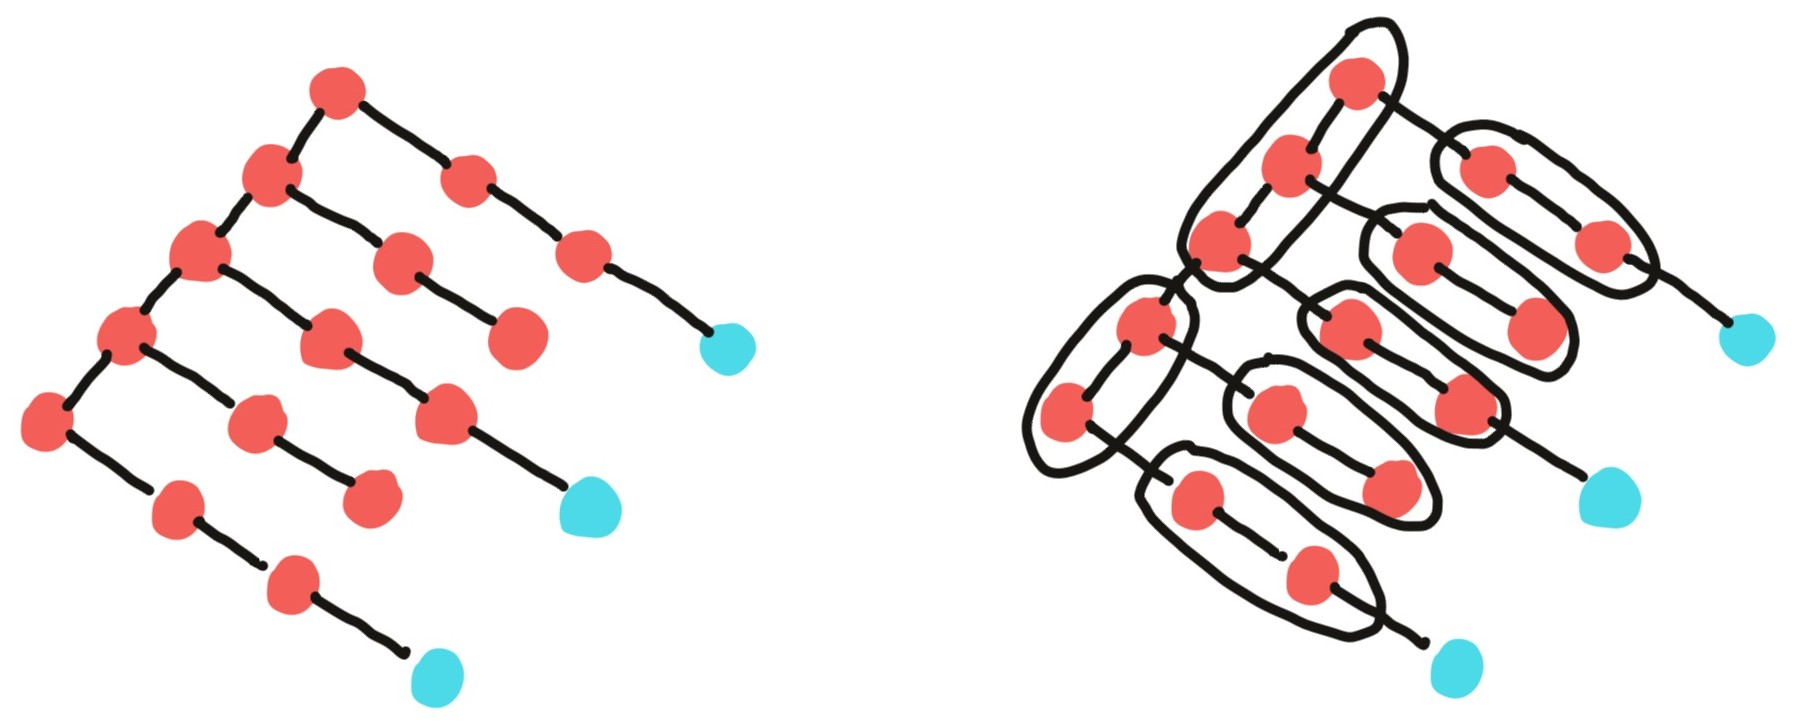
\includegraphics[scale=.15]{MyPic7.jpg}
\end{center}
Using similar arguments as befor, we can conclude that:
\begin{itemize}
\item The nodes inside $\rGamma$ factors have $\rGamma$ ancestors.  
\item If a $\ranked{\rSigma\setminus\rGamma}$ factor is the root of the factorized term, then its nodes do not have a $\rGamma$ ancestor.
\item   If a $\ranked{\rSigma\setminus\rGamma}$ factor is not the root of the factorized term, then its nodes do have a $\rGamma$ ancestor.
\end{itemize}
The ancestor function is obtained by applying $\ranked{\mathsf{root}_{f,g}}$ followed by a flattening.

Note here the importance of the basic function $\decfact$. If we had only the factorisation $\ancfact$, we would not be able to separate (at least easily) the red blocks having a blue descendent from the others in the figure above.  
\end{example}
%\medskip
%\noindent \begin{example}[Characteristic function of a finite type]
%Let $\rSigma, \Delta\in \Tt$ and suppose that $\rSigma$ is finite. 
%The order-preserving function $\chi_\rSigma:\Delta\to \llzero+\llone$ which satisfies $\chi_\rSigma(s)\in \llone$ if and only if $s\in \rSigma$ is a first-order tree function. 
%\end{example}
%\medskip
%\noindent \begin{example}[If then else] Suppose that $f : \rSigma \to \llzero+\llone$ and $g_0, g_1 : \rSigma \to\rGamma$ are first-order tree functions. Then the function:
% \begin{align*}
%  g\colon \rSigma &\to \rGamma \\
%  x &\mapsto g_0(x)  \text{ if } f(x)\in\llzero\\
%  x &\mapsto g_1(x)  \text{ if } f(x)\in\llone.
%\end{align*}
% is also a first-order tree function. This is done as follows. On input!!
%$x\in\rSigma$, we first apply the pairing of f and the identity function, yielding a result:
%$$ (f(x),x)\in(\llzero+\llone)\times\rSigma$$
%Next we apply the function distribute, transforming the type into:
%$$ \llzero\times\rSigma+\llone\times\rSigma$$
%To this result we apply the disjoint union $h_0 + h_1$ where $h_0:\llzero\times\rSigma\to \rGamma$ and
%$h_01:\llone\times\rSigma\to \rGamma$ are defined by $h_i=\pi_2(id_i,g_i)$, where $id_0$ and $id_1$ are the identity function on $\llzero$ and $\llone$ respectively, yielding the desired result.
%\end{example}

